% LaTeX Template for short student reports.
% Citations should be in bibtex format and go in references.bib
\documentclass[a4paper, 9pt]{article}
\usepackage[top=3cm, bottom=3cm, left = 2cm, right = 2cm]{geometry} 
\geometry{a4paper} 
\usepackage[utf8]{inputenc}
\usepackage{textcomp}
\usepackage{graphicx} 
\usepackage{amsmath,amssymb}  
\usepackage{bm}  
\usepackage[pdftex,bookmarks,colorlinks,breaklinks]{hyperref}  
\hypersetup{linkcolor=black,citecolor=black,filecolor=black,urlcolor=black} % black links, for printed output
\usepackage{memhfixc} 
\usepackage{pdfsync}  
\usepackage{fancyhdr}
\usepackage{fancyvrb}
\usepackage{natbib}
\usepackage{url}
%\pagestyle{fancy}
\usepackage{tabto}
\usepackage[shortlabels]{enumitem}
\usepackage{tikz}
\usepackage{verbatim}
\usepackage{nameref}
\usepackage{caption}
\usepackage{subcaption}

\begin{document}
\graphicspath{{./Images/}}
\begin{flushleft}

\section*{Sardines: A Networked Game}

\textit{Sardines} is a system of communication for 2-8 players. Each player controls a submarine in real time, viewing their surroundings through the lens of a retro sonar system. These submarines communicate in morse code, firing soundwaves - representative of dots and dashes - to one another across the map. While this system has ultimately been designed for integration into a larger, more complete game, \textit{Sardines} presents itself as a sandbox, to best restrict attention to the networking techniques at play.

\subsection*{Architecture}\label{Architecture}

\textit{Sardines}' network uses a straightforward client-server architecture, with the server's `master' game state well-positioned to minimise disputes (see `\nameref{Prediction}'). Furthermore, the architecture uses local input processing - each client takes responsibility for processing their own player's actions and transmitting the resulting changes, rather than leaving the central server to compute a new master state directly from raw input. This distributes the game's physics-based movement calculations in a far more even fashion; an authoritative server with less trust in the player would better prevent cheating \citep{gmbta10}, but `cheating' will be of little concern while \textit{Sardines} remains a sandbox game.
%Reasons for choice...
%Though the current system does not have many variables to keep track of, the server also provides a `master state' for clients to work from.
%Citation about networking [peer-reviewed]...

\vspace{5pt}\noindent
\citeauthor{bauer04} \citeyearpar{bauer04} evaluate the scalability of this architecture, finding that with $n$ entity states (for the purposes of the report, players), client-server costs grow at order $O(n^2)$, compared to peer-to-peer's $O(n^3)$. They ultimately conclude that ``The client-server architecture exhibits the lowest growth in overall system cost, however, with the disadvantage that the entire growth must be handled by the central server.''  

\vspace{5pt}\noindent
In light of their findings, this report proposes a hybrid architecture for \textit{Sardines} to adopt at scale. While it ultimately proved too ambitious for this assignment, the original idea for the game was that \textit{multiple} players work together in piloting each submarine: a co-operative exercise with a navigator relaying key information about the surroundings, and a small team of other crewmates individually controlling acceleration, steering, etc. With only navigators witnessing the global game state first-hand, Figure \ref{Hybrid Architecture} positions these clients as `local' servers, processing (up to, say) $3$ players' inputs simulataneously, and relaying major changes to the game state back down to this crew. Not only does this topology require less of the central server's bandwidth (it still maintains $2$-$8$ connections, while each navigator has up to $4$ and other crewmates exactly $1$),  but demands far less calculation than if all $32$ players send their highly-individualised updates directly to the master state.

\vspace{5pt}\noindent
\begin{figure}[h]
\centering
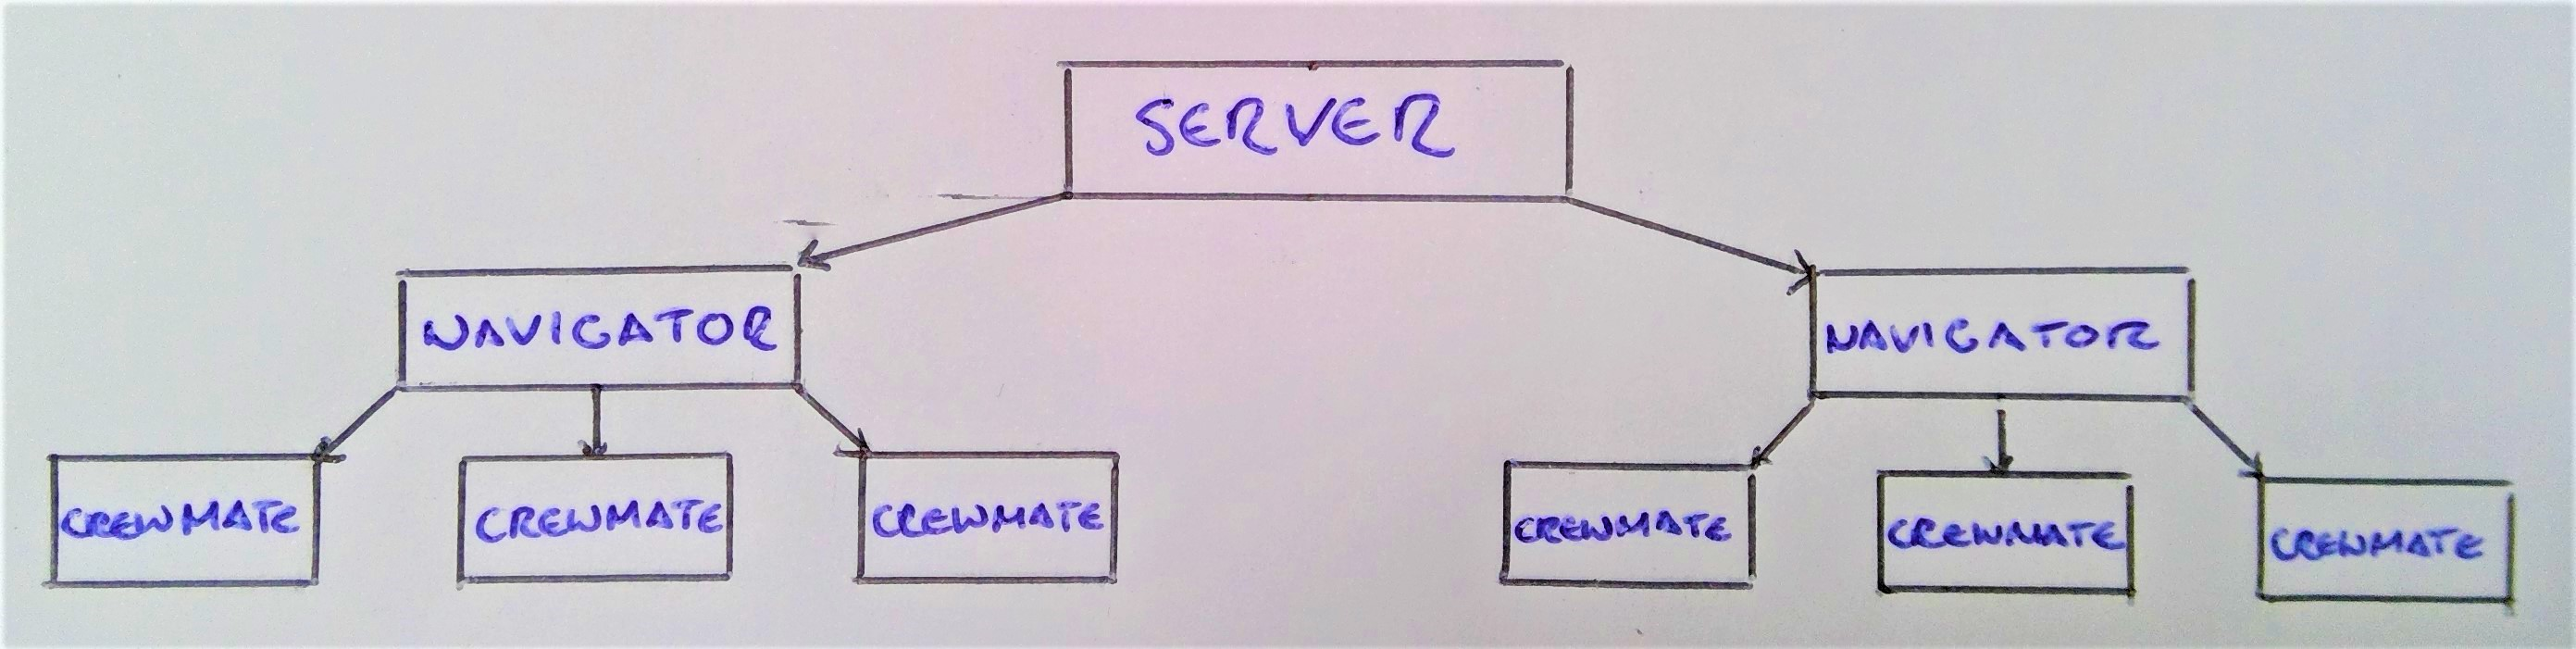
\includegraphics[width=0.85\textwidth]{Hybrid Architecture}
\caption{Potential hybrid architecture for a $32$-player version of \textit{Sardines} (simplified).}
\label{Hybrid Architecture}
\end{figure}

\subsection*{Protocols}

\paragraph{Transport Layer} In \textit{Sardines}, client and server communicate through TCP connections, chosen for their reliability. 
As much is set out in RFC 798 \citeyearpar{rfc793}, where \citeauthor{rfc793} introduces the protocol:.... %`` ''
Provide reliability paragraph?...

\vspace{5pt}\noindent
There is, of course, an argument for updating positions via UDP. Suppose that a submarine starts at position $A$, fails to update to position $B$: where the ordered nature of TCP means the application will resend and resend this update [EXPLAIN DOWNSIDE], this protocol will simply [GO TO the position C of the next successful].  While the deliberate simplicity of UDP - the [FEATURE \#1], the [FEATURE \#2] - lends itself to the continuous, incremental nature of movement , \textit{Sardines} will not make use of it. Submarines in this game travel slowly, with positions needed reliably but not immediately, and with the robustness of the prediction system used (see `\nameref{Prediction}'), updating position via TCP every 0.1s should be infrequent enough to avoid the backlog described above.

\paragraph{Application Layer} 

While it needn't consider the internetwork and hardware layers of the protocol stack, the application layer of \textit{Sardines}' network necessarily interacts with the transport layer directly below it. Data is sent via \texttt{SendablePacket}s, consisting of a fixed-length \texttt{HeaderPacket} and one of several structs encoded as a \texttt{serialisedBody}. The header, always read first, contains a \texttt{bodyID}  that tells the receiver how many bytes of the body need deserialised; as discussed in the labs, this application handles variable-length messages in much the same way as the DNS protocol.

\vspace{5pt}\noindent
At a more granular level, a \texttt{serialisedBody} may encode one of many structs, for one of many purposes:
\begin{itemize}[noitemsep]
\item \texttt{SyncPacket} Contains a \texttt{long} \texttt{syncTimestamp}. Sent on connection to standardise server and client calculations for \texttt{DateTime.UtcNow.Ticks} (which may vary from underlying OS to underlying OS, \citealp{msftUTC}).
\item \texttt{IDPacket} Contains an \texttt{int} \texttt{clientID}, and a \texttt{char[]} \texttt{clientIP} that requires, by definition, no more than $16$ characters. Sent to initialise a unique identity for each client, and more generally let players track who else is playing.\footnote{In the hybrid architecture discussed above, the IP would also be used to establish crew-to-navigator connections.}
\item \texttt{SubmarinePacket} Contains an \texttt{int} \texttt{submarineID}, the controller's \texttt{clientID}, and additional variables corresponding to future functionalities. Similarly initialises a unique identity for each submarine.\footnote{And similarly, the distinction between \texttt{clientID} and \texttt{submarineID} is only meaningful, of course, with multiple clients per submarine.}
\item \texttt{PositionPacket} Contains a submarine's \texttt{x}-, \texttt{y}-coordinates and rotation \texttt{theta} at a certain time \texttt{timestamp}. Sent client-to-server as updates to the master game state, and server-to-client for prediction and rendering.
\item \texttt{MorsePacket} Similarly contains the necessary parameters to render a soundwave's arc on the receiving client's screen.
\item \texttt{EmptyPacket} Contains no variables. Sent when the \texttt{bodyID} corresponds to a function with no arguments (e.g. \texttt{bodyID} \texttt{2310} tells a server in lobby mode to initialise a game).
\end{itemize}
\texttt{bodyID}s adopt an informal naming convention: IDs \texttt{1XXX} refer to clients connecting to/disconnecting from a server, \texttt{2XXX} to server functionality while in lobby mode, \texttt{3XXX} to server functionality while in a game mode, and \texttt{4XXX} to client states and actions while in-game.

\vspace{5pt}\noindent
While there isn't the space to break down every protocol in precise detail, all have been designed with the same underlying philosophy. Consider, for instance, the process of joining a lobby:
\begin{enumerate}[label=\textit{\arabic*}\textit{.}, noitemsep]
\item \textit{The client registers a TCP connection with the server.} The client then constructs... with ID \texttt{1000}...
\item \textit{The server receives a \texttt{SyncPacket} from the client.} Calling \texttt{Receive1000()}, the server...
\item \textit{The client receives a \texttt{SyncPacket} from the server.}
\item \textit{The server receives an \texttt{IDPacket} from the client.}
\item \textit{The client receives an \texttt{IDPacket} from the server.}
\item \textit{All clients receive (further) \texttt{IDPacket}s from the server.}
\end{enumerate}
There is arguably some unnecessary back-and-forth to the above, but small packet sizes shouldn't put any meaningful strain on bandwidth. The process is designed for ease of programming: treating major protocols as a chain of smaller, simpler steps, it becomes far easier to manage - and document - the application layer. 
%This description may seem fairly dry, but it serves to ...
%There is some degree of back-and-forth to this process...


\subsection*{API}

% CHECKME: What is an API?
\textit{Sardines} is built with C\# in the Godot engine. It uses System.Net.Sockets to handle networking, and System.Runtime.InteropServices to serialize/deserialize packet structs. As noted in Microsoft's documentation \citeyearpar{msftSNS}, System.Net.Sockets implements conventional Berkeley sockets.



\pagebreak
\subsection*{Integration}

Asynchronous I/O...
Connection class...

\vspace{5pt}\noindent
Discuss: offline vs. online updates to position!

\vspace{5pt}\noindent
This report would be amiss to skip over the final step: 

\subsection*{Prediction}\label{Prediction}

As discussed under `\nameref{Architecture}',  clients only send position updates every $0.1s$. What this report has so far failed to consider is how this appears to other clients - they experience what should be a smooth, continuous movement as discontinuous jumps over $0.1s$ intervals! Clearly, ... [introduce prediction - with reading?].

\vspace{5pt}\noindent
When a player chooses to move forward, they do not jump to a constant speed but continuously accelerate from zero; naturally, \textit{Sardines} uses second-order quadratic prediction to best approximate the second-order derivative of accelaration. Given a submarine's three most recent positions $\mathbf{r}_0$, $\mathbf{r}_1$,$\mathbf{r}_2$ (corresponding to times $t_0 > t_1 > t_2$), clients can average the velocities from $\mathbf{r}_1$ to $\mathbf{r}_0$, from $\mathbf{r}_2$ to $\mathbf{r}_1$, and the acceleration from $\mathbf{r}_1$ to $\mathbf{r}_0$ as
$$\mathbf{u}_0 = \frac{\mathbf{r}_0-\mathbf{r}_1}{t_0-t_1}, \;\; \mathbf{u}_1 = \frac{\mathbf{r}_1-\mathbf{r}_2}{t_1-t_2}, \;\; \mathbf{a}_0 = \frac{\mathbf{u}_0-\mathbf{u}_1}{t_0-t_1}, \;\; \textrm{respectively.}$$
These estimates define the quadratic model
$$ \mathbf{\tilde{r}}(t) = \mathbf{r}_0+\mathbf{u}_0t+\mathbf{a}_0t^2.$$
%FIXME: Subject to experiementation!
In contrast, the rudder controlling a submarine's rotation $\theta$ \textit{is} controlled at a constant speed, so \textit{Sardines} only uses linear prediction to approximate
$$\mathbf{\tilde{\theta}}(t) = \mathbf{\theta}_0+\mathbf{\dot{\theta}}_0t$$
(with subtle, case-specific considerations made given $\theta \in [0,2\pi)$).


\vspace{5pt}\noindent
If prediction is the act of waiting for data, then integration is how one `catches up' on receiving it. On receiving a new \texttt{PositionPacket} at time $t_0$, a programmer might be inclined to start predicting under to a new quadratic model $\mathbf{\tilde{r}}_{\textrm{new}}(t)$ immediately, but if positions $\mathbf{\tilde{r}}_{\textrm{old}}(t_0)$ and $\mathbf{\tilde{r}}_{\textrm{new}}(t_0)$ are visibly far apart, then the player will see the corresponding submarine make an instantaneous jump across the screen.\footnote{This might be regarded interpolation over $T = 0.0s$!} Instead, one takes a set time $T$ to linearly interpolate from the old trajectory to the new:
$$\mathbf{\tilde{r}}(t) = \begin{cases} 
\mathbf{\tilde{r}}_{\textrm{old}}(t) & \textrm{if $t < t_0$} \\
(1-q(t))\mathbf{\tilde{r}}_{\textrm{old}}(t) + q(t)\mathbf{\tilde{r}}_{\textrm{new}}(t) & \textrm{if $t_0 \leq t < t_0+T$} \\
\mathbf{\tilde{r}}_{\textrm{new}}(t) & \textrm{if $t \geq t_0+T$}
\end{cases}, \;\; \textrm{where $q(t) = \frac{1}{T}\left(t-t_0\right)$.}$$
In \textit{Sardines}' particular implementation, \texttt{PositionPacket}s are sent via TCP every $0.1s$; interpolation therefore takes place over a strictly shorter interval $T = 0.05s$. 
%Footnote - quirk of how we deal with being two packets behind?

\begin{figure}[h]
\centering
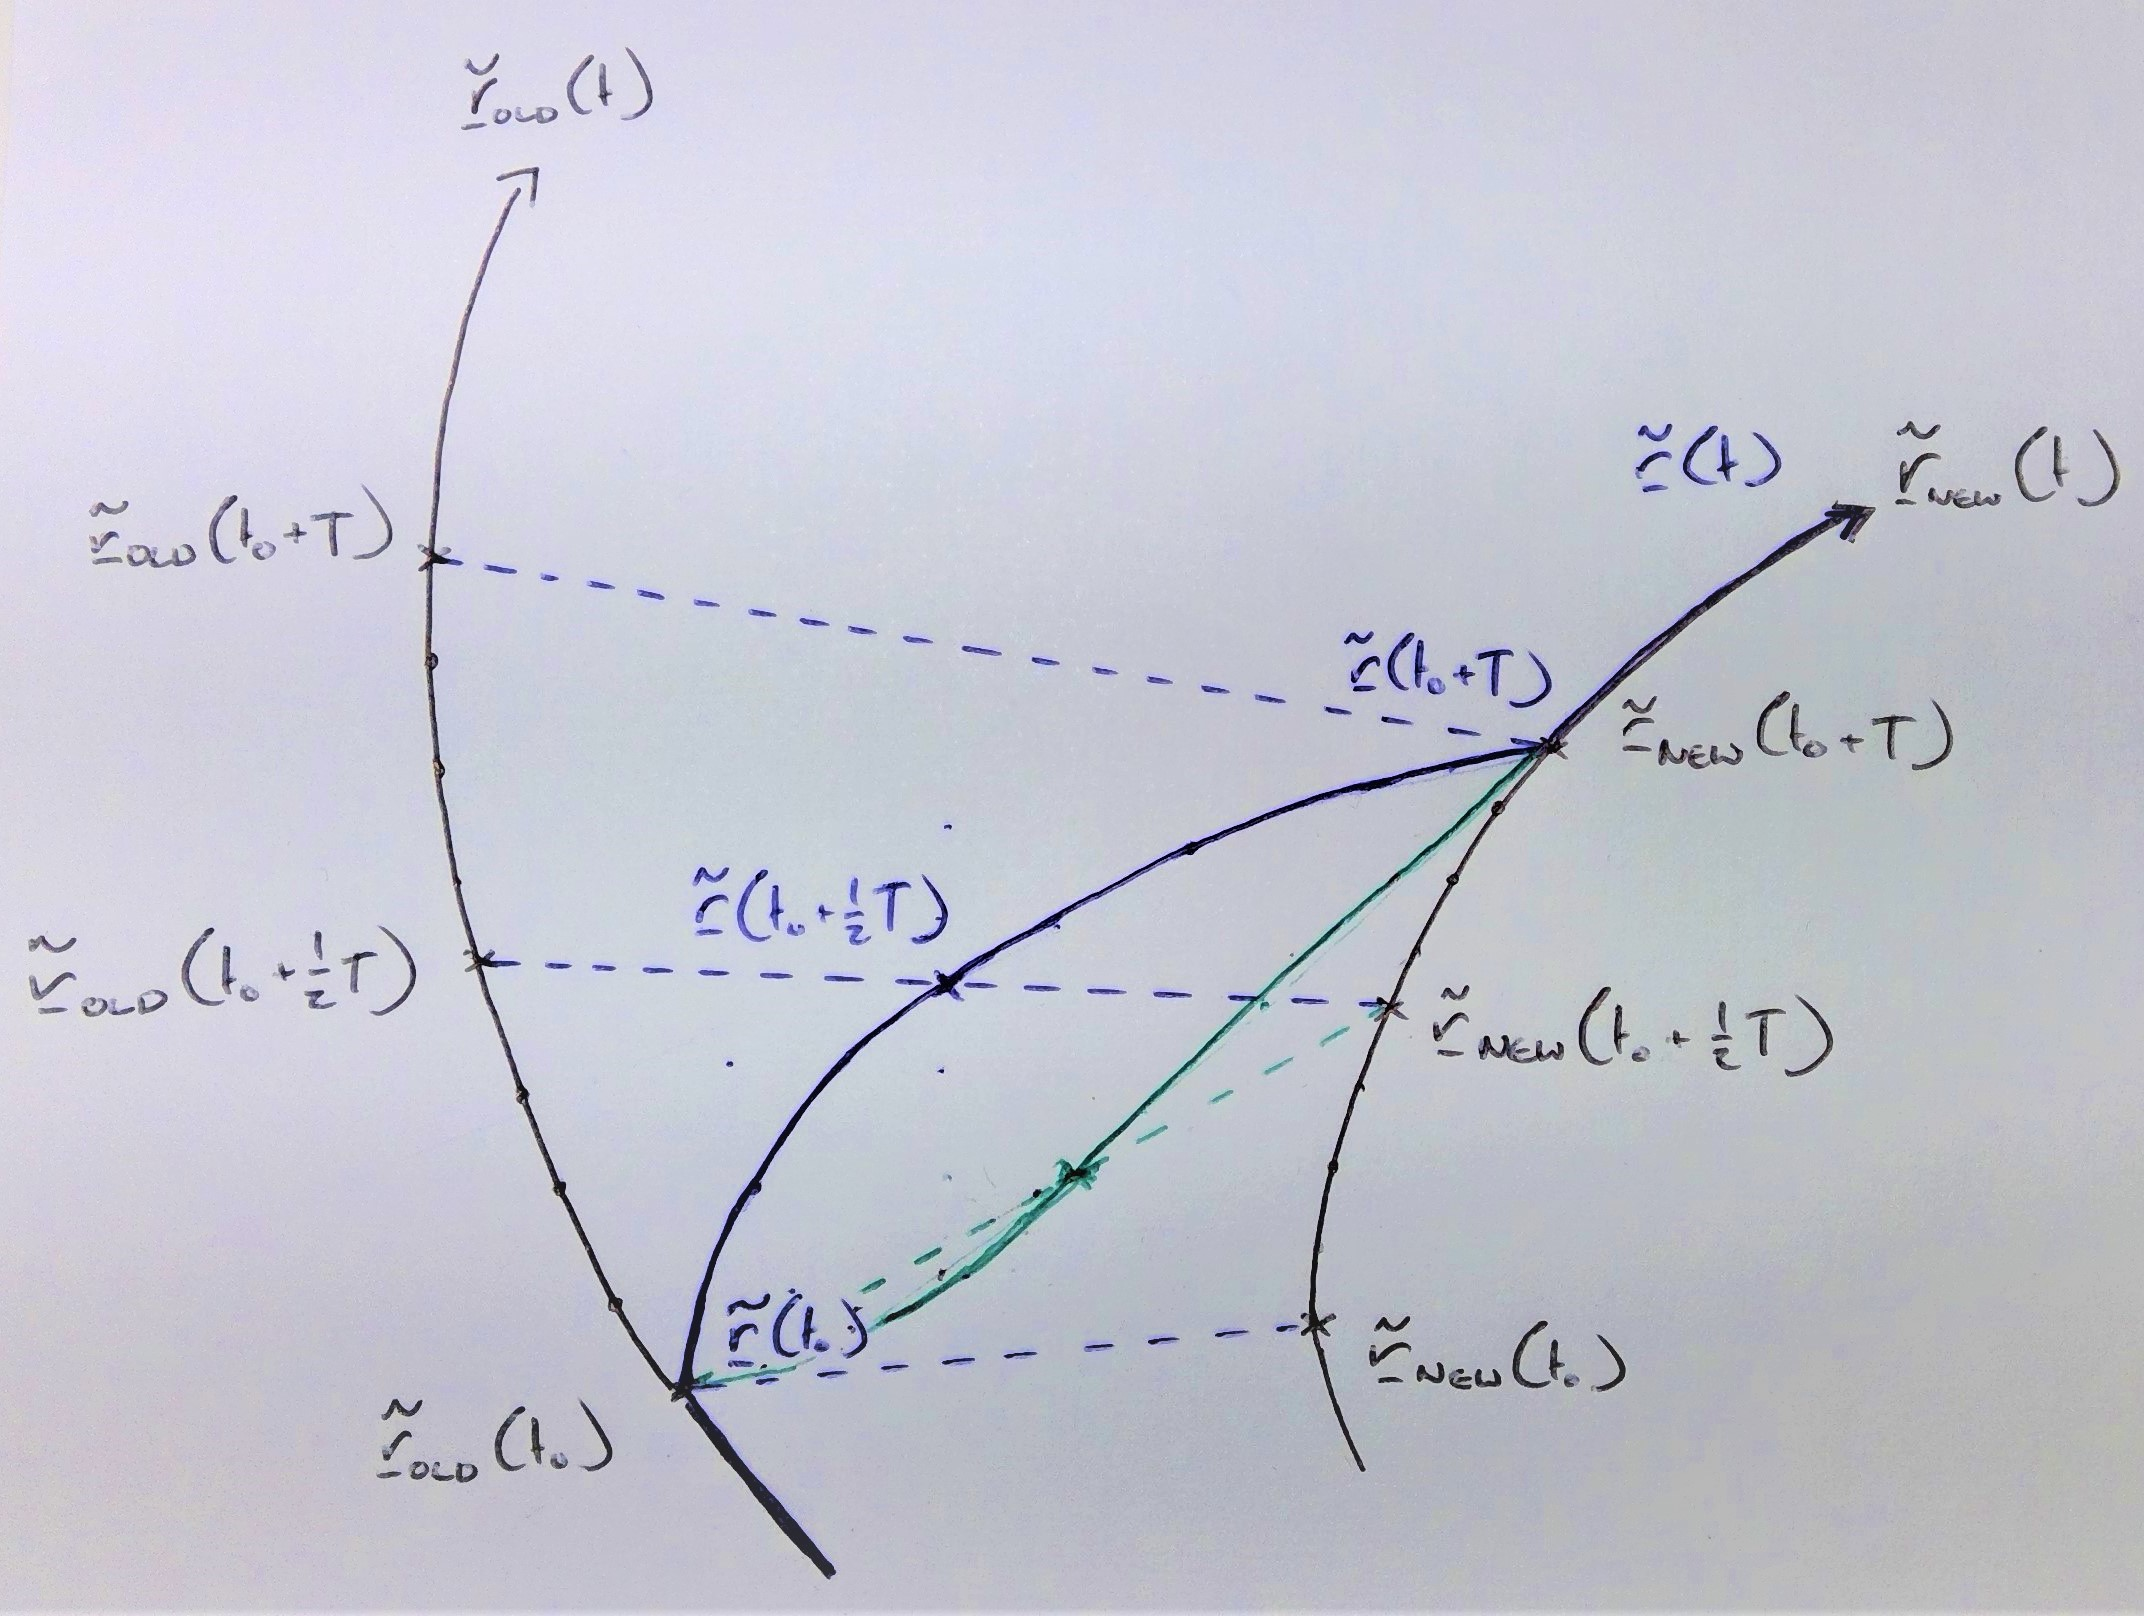
\includegraphics[width=0.85\textwidth]{Interpolation}
\caption{Interpolation from trajectory $\mathbf{\tilde{r}}_{\textrm{old}}(t)$ to $\mathbf{\tilde{r}}_{\textrm{new}}(t)$ (blue); chosen over $\mathbf{\tilde{r}}_{\textrm{old}}(t_0)$ to $\mathbf{\tilde{r}}_{\textrm{new}}(t)$ (red).}
\label{Interpolation}
\end{figure}

To fully understand how \textit{Sardines} uses it prediction techniques, this report must first introduce a core challenge of any networked game: conflict resolution.

\vspace{5pt}\noindent
In \textit{Sardines}, the projectiles concerned are soundwaves. The visual language of the game, where soundwaves from external sources only become visible on collision with the player, provides a clear approach: the sender unequivocally takes precedence. Only when a player sees their soundwave hit another is a \texttt{MorsePacket} sent from their client (which will arrive with the usual delay). The sender knows with certainty who receives their message; the receiver, who cannot see the trajectory of the soundwave until it arrives, will have no sense of whether it ``should'' have hit them.

\vspace{5pt}\noindent
To further `smooth over' the application's conflict resolution, the receiving client makes use of backward prediction. Since neither server nor client stores more than three of any submarine's past positions at a time, it is fortunate the above formulae can approximate the past as well as the future.\footnote{\textit{Sardines}' submarines are physics-based objects, and at one point in development, the drag they experience was factored into prediction. However, the differential equations for 2D motion with a quadratic drag were too complex to find an analytic solution - rather than being able to substitute a $t$-value into a given equation, the prediction would be calculated over incremental, irreversible forward time steps - so the application sacrifices this more realistic model for the ability to look backwards in time.}

\vspace{5pt}\noindent
Suppose a sender emits a soundwave from position $\mathbf{r}$ at time $t_0$, which they see reach a receiver at $t_0+\Delta t$. On the arrival of the corresponding packet at $t_1$, then, the receiving client has to decide where the wave was emitted from \textit{in its local view of the game}. The obvious choice would be the `true origin' $\mathbf{r}$, but \textit{Sardines} uses the backwards prediction $\mathbf{\tilde{r}}(t_1-\Delta t)$. As [FIGURE] puts it in [REFERENCE], [QUOTE]; conflict resolution is the art of deciding which quantities are preserved across clients, and \textit{Sardines} - a system designed around slow, real-time communications - is far less concerned with a shared view of geography than it is a shared view of delay.

\pagebreak
\subsection*{Testing}

\vspace{5pt}\noindent
[PARAGRAPH OF METHODOLOGY]
Using clumsy...
Since \textit{Sardines} only uses TCP connections, it ; this report will restrict its analysis to performance under latency and throttle

\paragraph{Latency} Latency (or, colloquially, lag) is...
For a game being released at scale, it is recommended to test latencies from $100ms$ to $1000ms$, as a bare minimum \citep{unityNTWK}.

\begin{figure}[h]
\centering
\caption{Three simultaneous, local views of the game world, at [ACCEPTABLE LAG]$ms$ lag (above); [UNACCEPTABLE LAG]$ms$ lag (below).}
\label{Lag Testing}
\end{figure}

\vspace{5pt}\noindent
[Paragraph of Evaluation] The choice of a TCP as the application's sole transport protocol is seems to be of [little/significant] disadvantage here. [Central idea: design decisions that seem optimal in theory, but need tested in practice!]

\paragraph{Throttle} [EXPLANATION OF THROTTLE AND TESTING]

\vspace{5pt}\noindent
Testing lag and throttle simultaneously yields unsurprising results. Having established acceptable network conditions - [TIME]$ms$ lag, a [$\%$ chance of [TIME]$ms$ throttle -

\vspace{5pt}\noindent
Recall the interpolation technique described above. Since $T < 0.1s$, the report has assumed the submarine being interpolated appears at position starts on a predicted trajectory at time $t_0$ - does this assumption hold in practice? If two \texttt{PositionPacket}s have been throttled, and arrive within $T$ seconds of each other, it follows that the submarine will not have finished its first interpolation by the time the second one starts! In this edge case of being caught mid-interpolation at some point $\mathbf{r}_0$, \textit{Sardines} prioritises catching up; rather than using a predicted trajectory as in Figure \ref{Interpolation}, the subsequent interpolation simplifies calculations by taking $\mathbf{\tilde{r}}_{\textrm{old}}(t) = \mathbf{r}_0$.

\vspace{5pt}\noindent
Indeed, for all the optimisations and oversights discussed in this section, its worth noting how fundamental testing has already been in development. With network programming being notoriously unpredictable, \textit{Sardines} has necessarily involved a lot of QA: a feature that works offline must be tested between a single client and the server; then between two clients on the same device; then across devices, or between more clients, or under poor network conditions; the list goes on. While [Conclude here, or one final paragraph for more general reflection?].

\bibliographystyle{agsm}
\bibliography{References}
\end{flushleft}
\end{document}

